\begin{itemize}
    \item In der Regel ist zumindest ein kurzes Theoriekapitel notwendig. Es nimmt Bezug auf das thematische Oberthema, aber natürlich nicht auf allgemeine theoretische Grundlagen etwa aus der Naturwissenschaft.
\end{itemize}

\section{Formula SAE Competitions}
The main idea of a Formula SAE competition is to conceive, design, fabricate, develop and compete with small, formula style, race cars.
The competition is split into two classes: Internal Combustion Engine Vehicle (\acrshort{cv}) and Electric Vehicle (\acrshort{ev}).
Additionally, a team can opt-in to take part in the Driverless Cup (\acrshort{dc}).
After a series of technical inspections in regards for safety and rules compliance, the vehicles will then compete in a series of static and dynamic events. In the end, the team with the most overall points will win the competition for its class or the \acrlong{dc}, respectively. \cite{fs_rules_2022_handbook}
\begin{figure}[H]
    \centering
    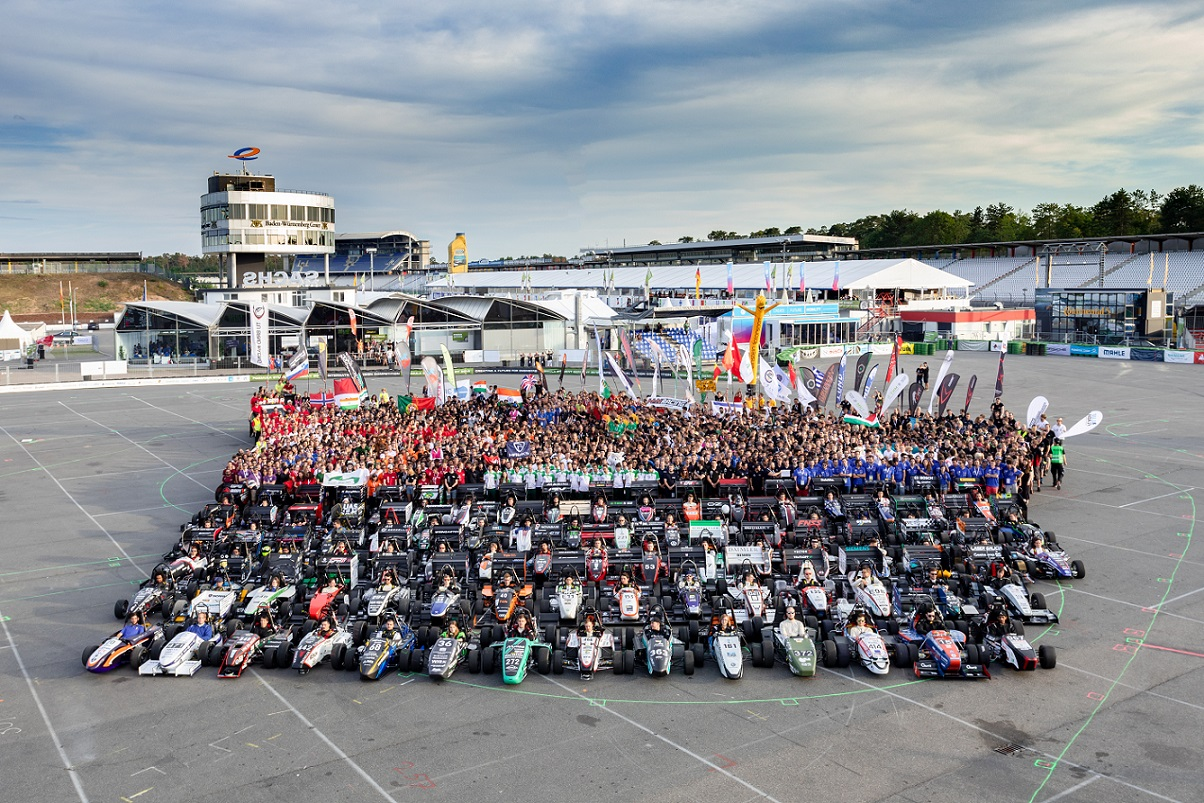
\includegraphics[width=\columnwidth]{FS_SAE_Competition.jpeg}
    \caption{Teams participating at Formula Student Germany ©FS Germany}
    \label{fig:FS SAE Competition}
\end{figure}

\subsection{Static Events}
The following static events are held: Business Plan Presentation, Cost and Manufacturing, and Engineering Design. In these events, the engineers have to present their car and their development processes to a panel of judges. \cite{fs_rules_2022_handbook}

\begin{itemize}
    \item \textbf{Business Plan Presentation:} The team's ability to develop and deliver a comprehensive business model will be evaluated. The presentation should demonstrate how their self-developed race car could become a profitable business idea.
    \item \textbf{Cost and Manufacturing:} The financial planning of the car, including the manufacturing processes and costs associated with the construction of the race car are evaluated.
    \item \textbf{Engineering Design:} Evaluation of the engineering process and effort that went into the design of the vehicle. Technical aspects, the construction and key attributes of the car will be judged.
\end{itemize}

\subsection{Dynamic Events}
The following dynamic events are held: Skid Pad, Acceleration, Autocross, Endurance and Efficiency, and Trackdrive.
The dynamic events reveal the driving performance of the prototypes. Every discipline puts different abilities of the cars to the test. \cite{fs_rules_2022_handbook}
\begin{itemize}
    \item \textbf{Skid Pad:} The skid pad track consists of two pairs of concentric circles in the shape of an eight. This track will test the lateral grip of the car.
    \begin{figure}[H]
        \centering
        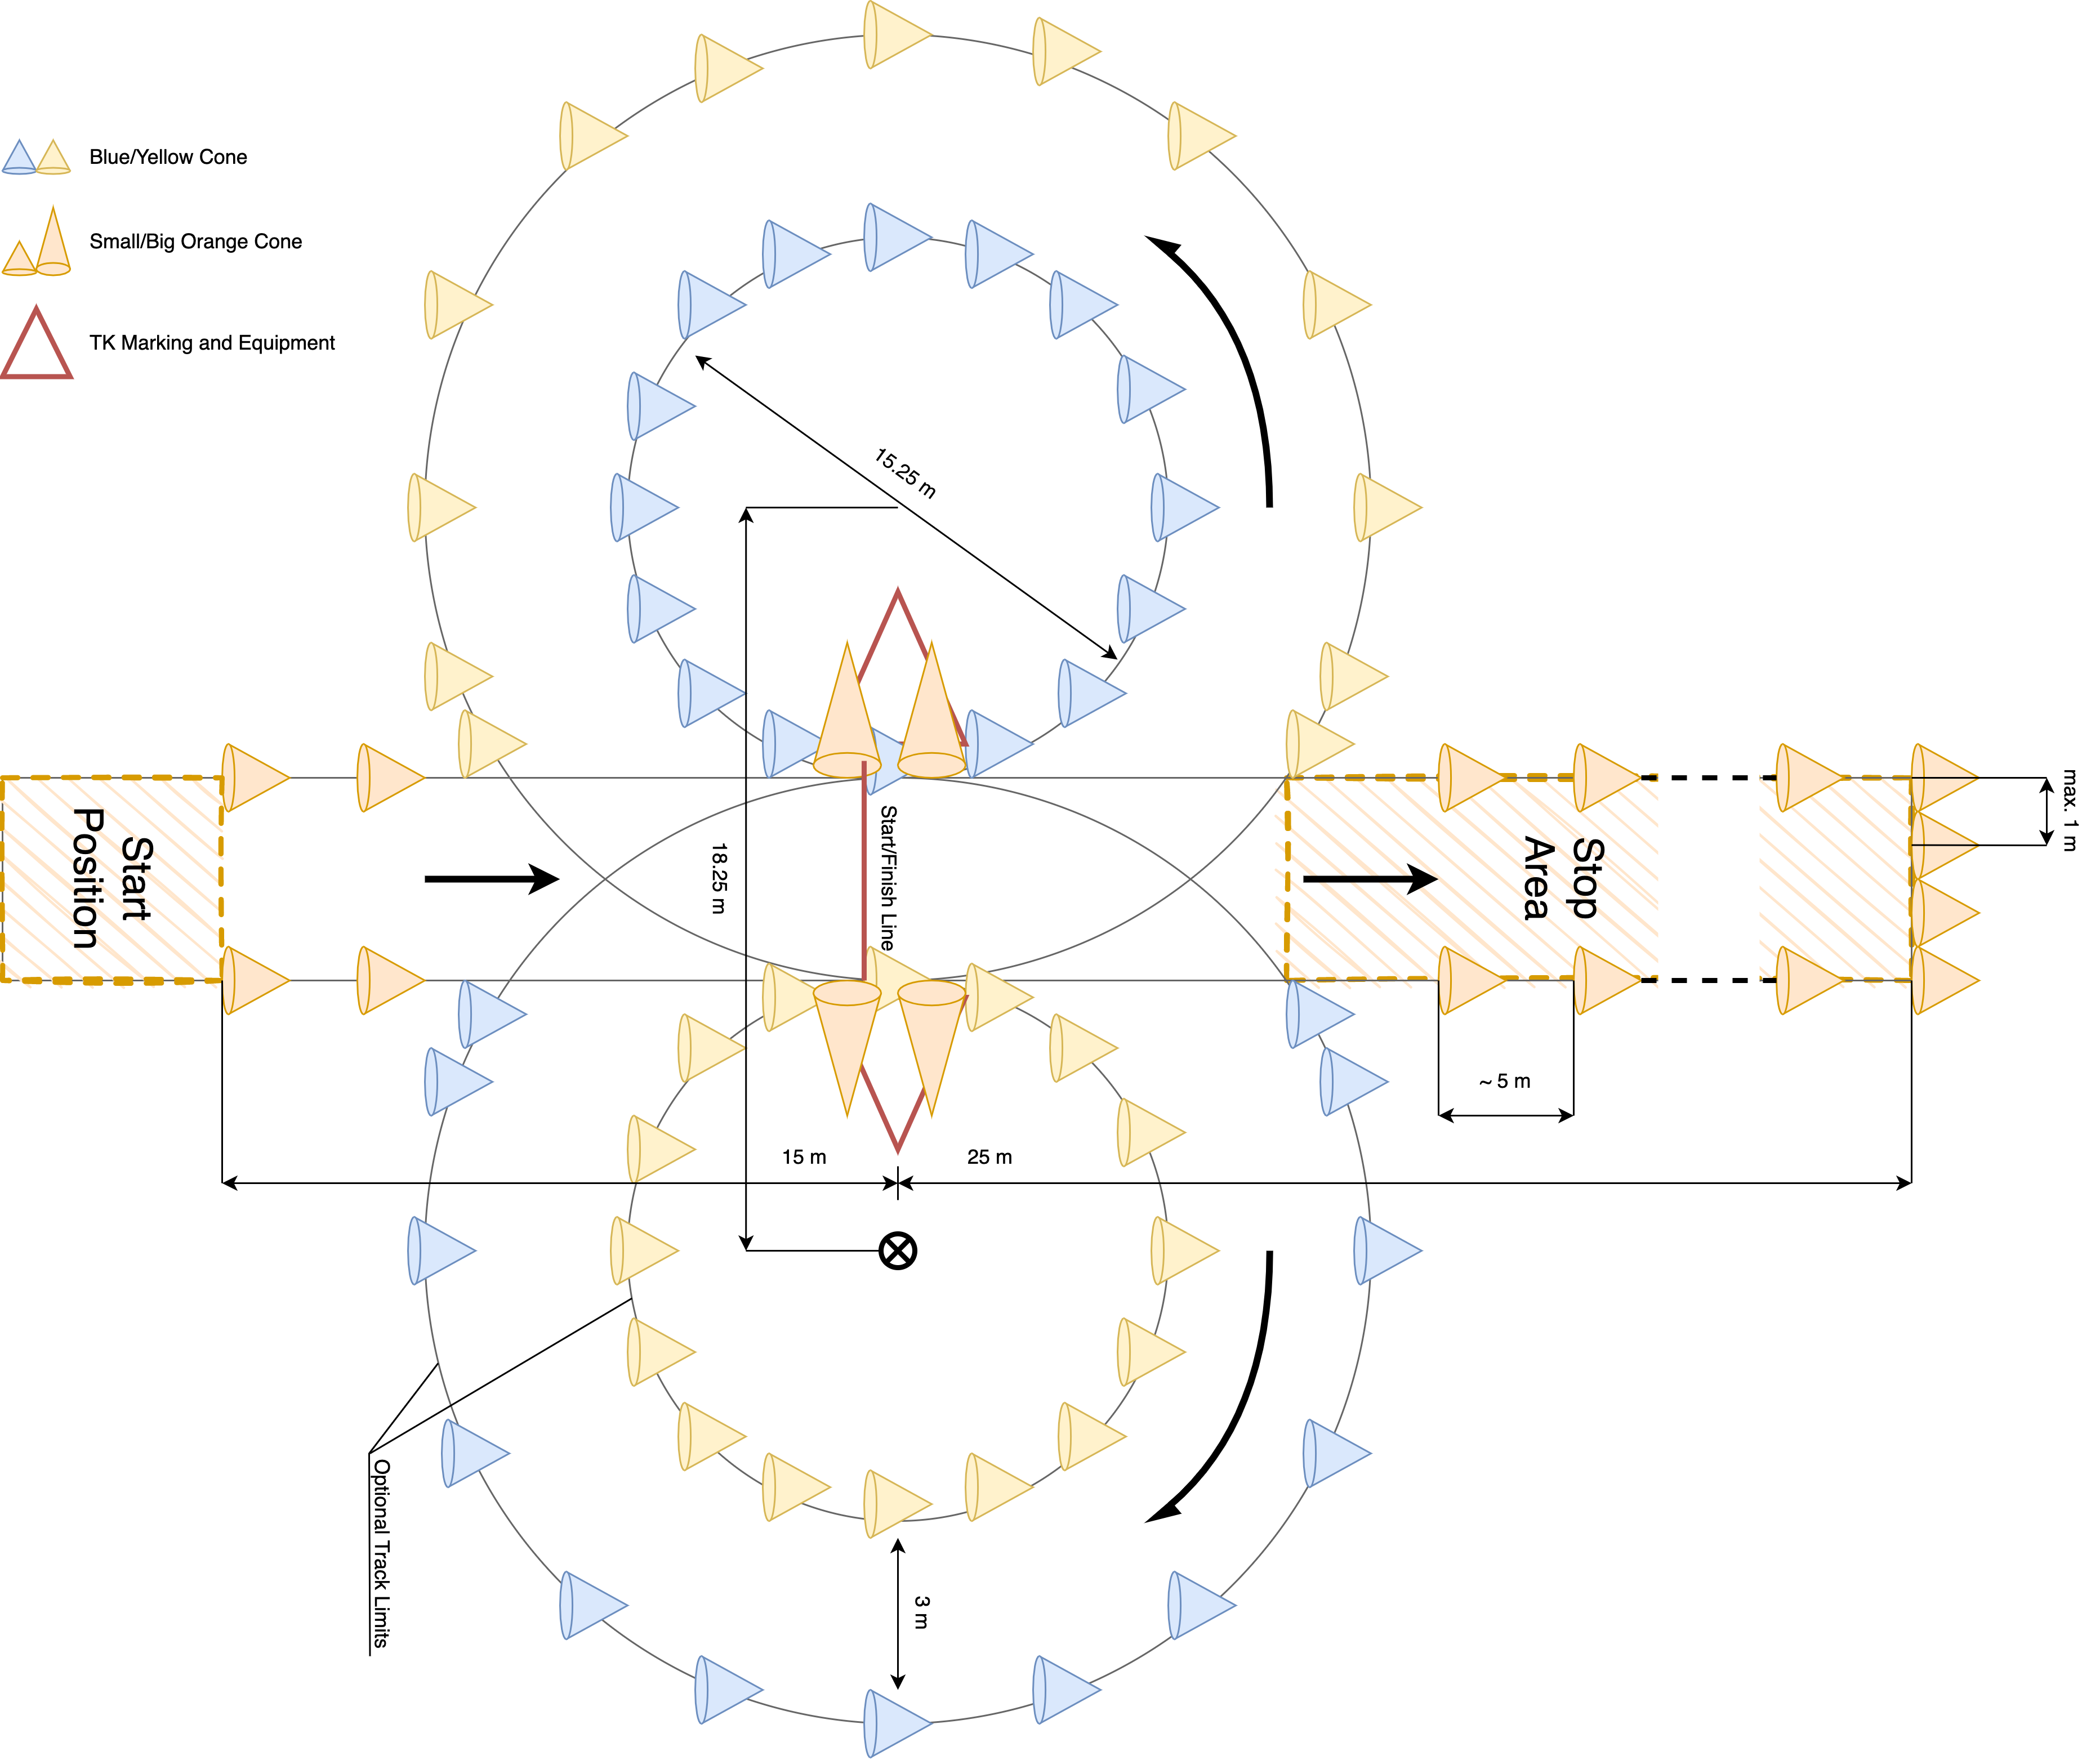
\includegraphics[width=\columnwidth]{FS_Event_Skid_Pad.png}
        \caption{Skid Pad track layout according to section D4 in the Formula Student Rules 2022 handbook \ref{fs_rules_2022_handbook}.}
        \label{fig:FS Skid Pad layout}
    \end{figure}
    \item \textbf{Acceleration:} An acceleration race over 75 m distance with a standing start, which tests the car acceleration in a straight line.
    \begin{figure}[H]
        \centering
        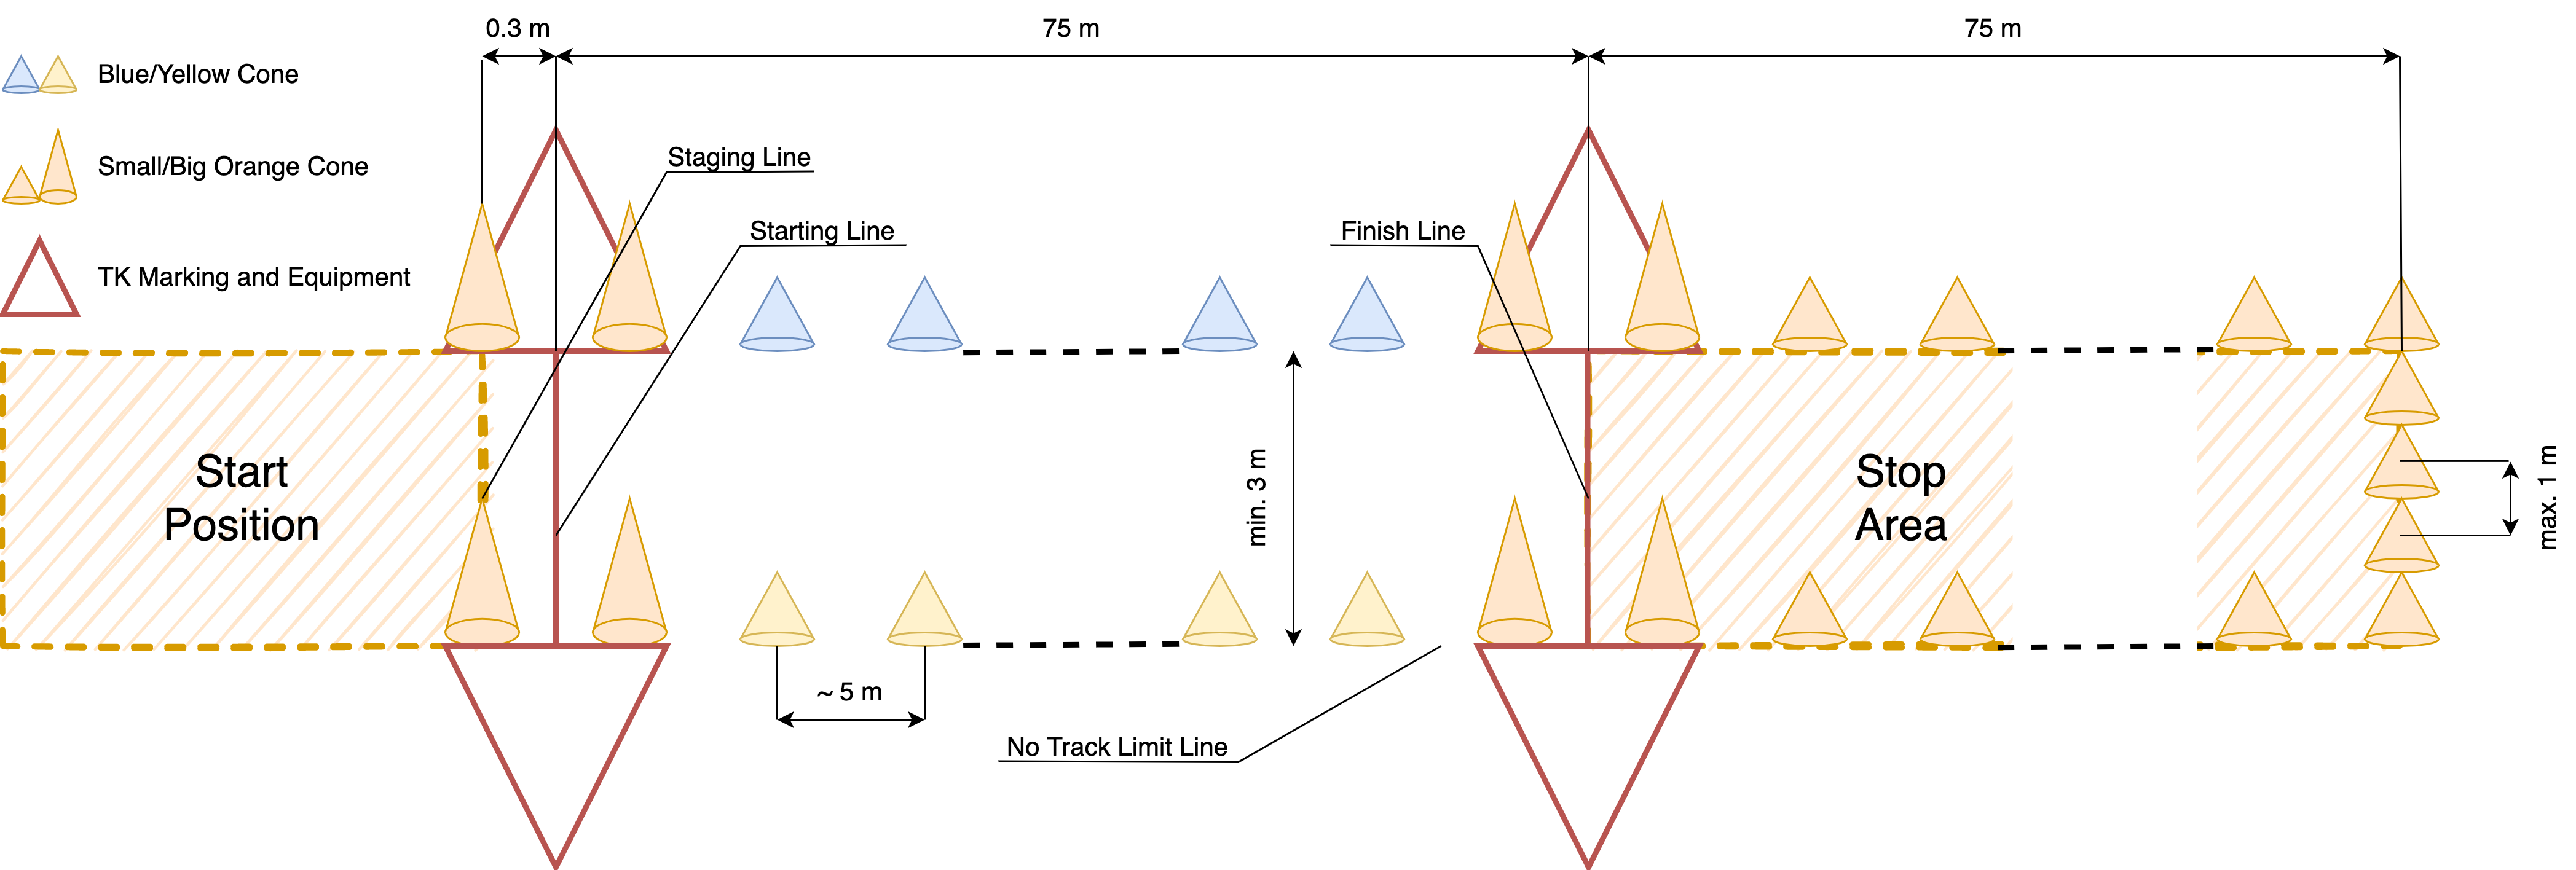
\includegraphics[width=\columnwidth]{FS_Event_Acceleration.png}
        \caption{Acceleration track layout according to section D5 in the Formula Student Rules 2022 handbook \ref{fs_rules_2022_handbook}.}
        \label{fig:FS Acceleration layout}
    \end{figure}
    \item \textbf{Autocross:} The autocross event tests the cars dynamic ability in a one lap sprint. The objective of the autocross event is to evaluate the car's manoeuvrability and handling qualities.
    \item \textbf{Endurance and Efficiency:} An endurance race over a distance of 22 km, including one driver change. One lap of the endurance track is approximately 1 km. The Efficiency scoring rates the consumed amount of energy in relation to the total time.
    \item \textbf{Trackdrive (DC Only):}  Over a distance of 10 rounds, the car has to prove its durability without a driver under long-term conditions.
    \begin{figure}[H]
        \centering
        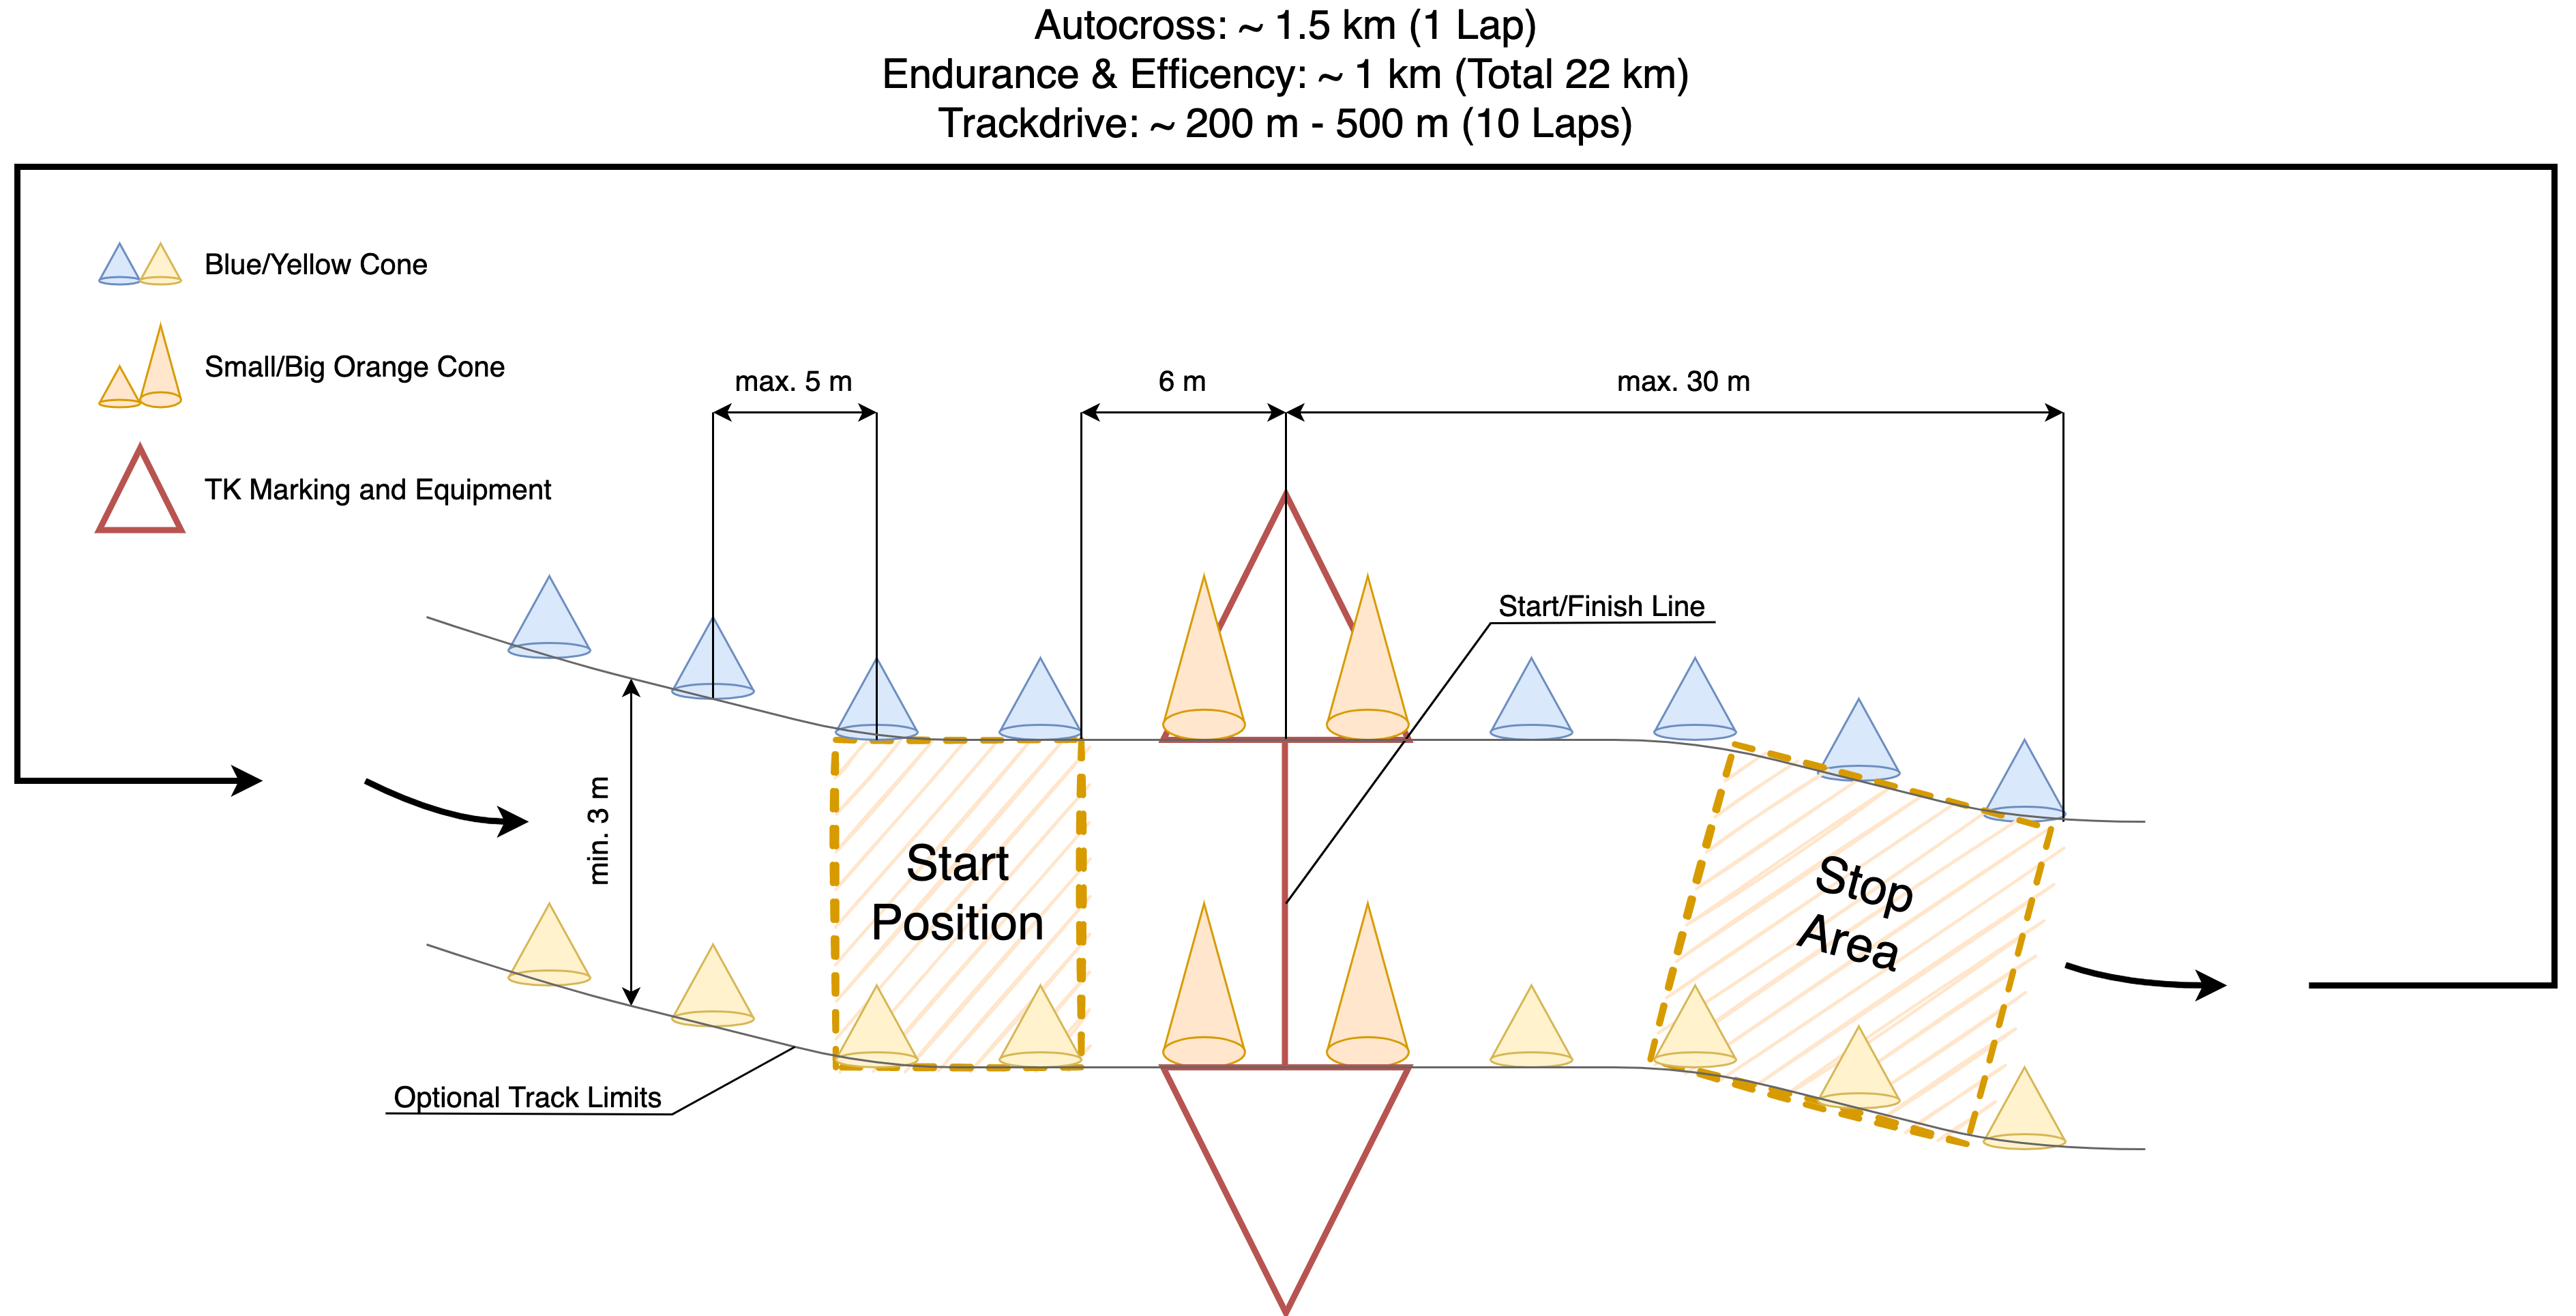
\includegraphics[width=\columnwidth]{FS_Event_Trackdrive.png}
        \caption{Base layout for the Autocross, Endurance and Trackdrive events according to sections D6, D7 and D8 in the Formula Student Rules 2022 handbook \ref{fs_rules_2022_handbook}.}
        \label{fig:FS Autocross, Endurance and Trackdrive layout}
    \end{figure}
\end{itemize}

\section{Zurich UAS Racing Autonomous System}
\begin{figure}[H]
    \centering
    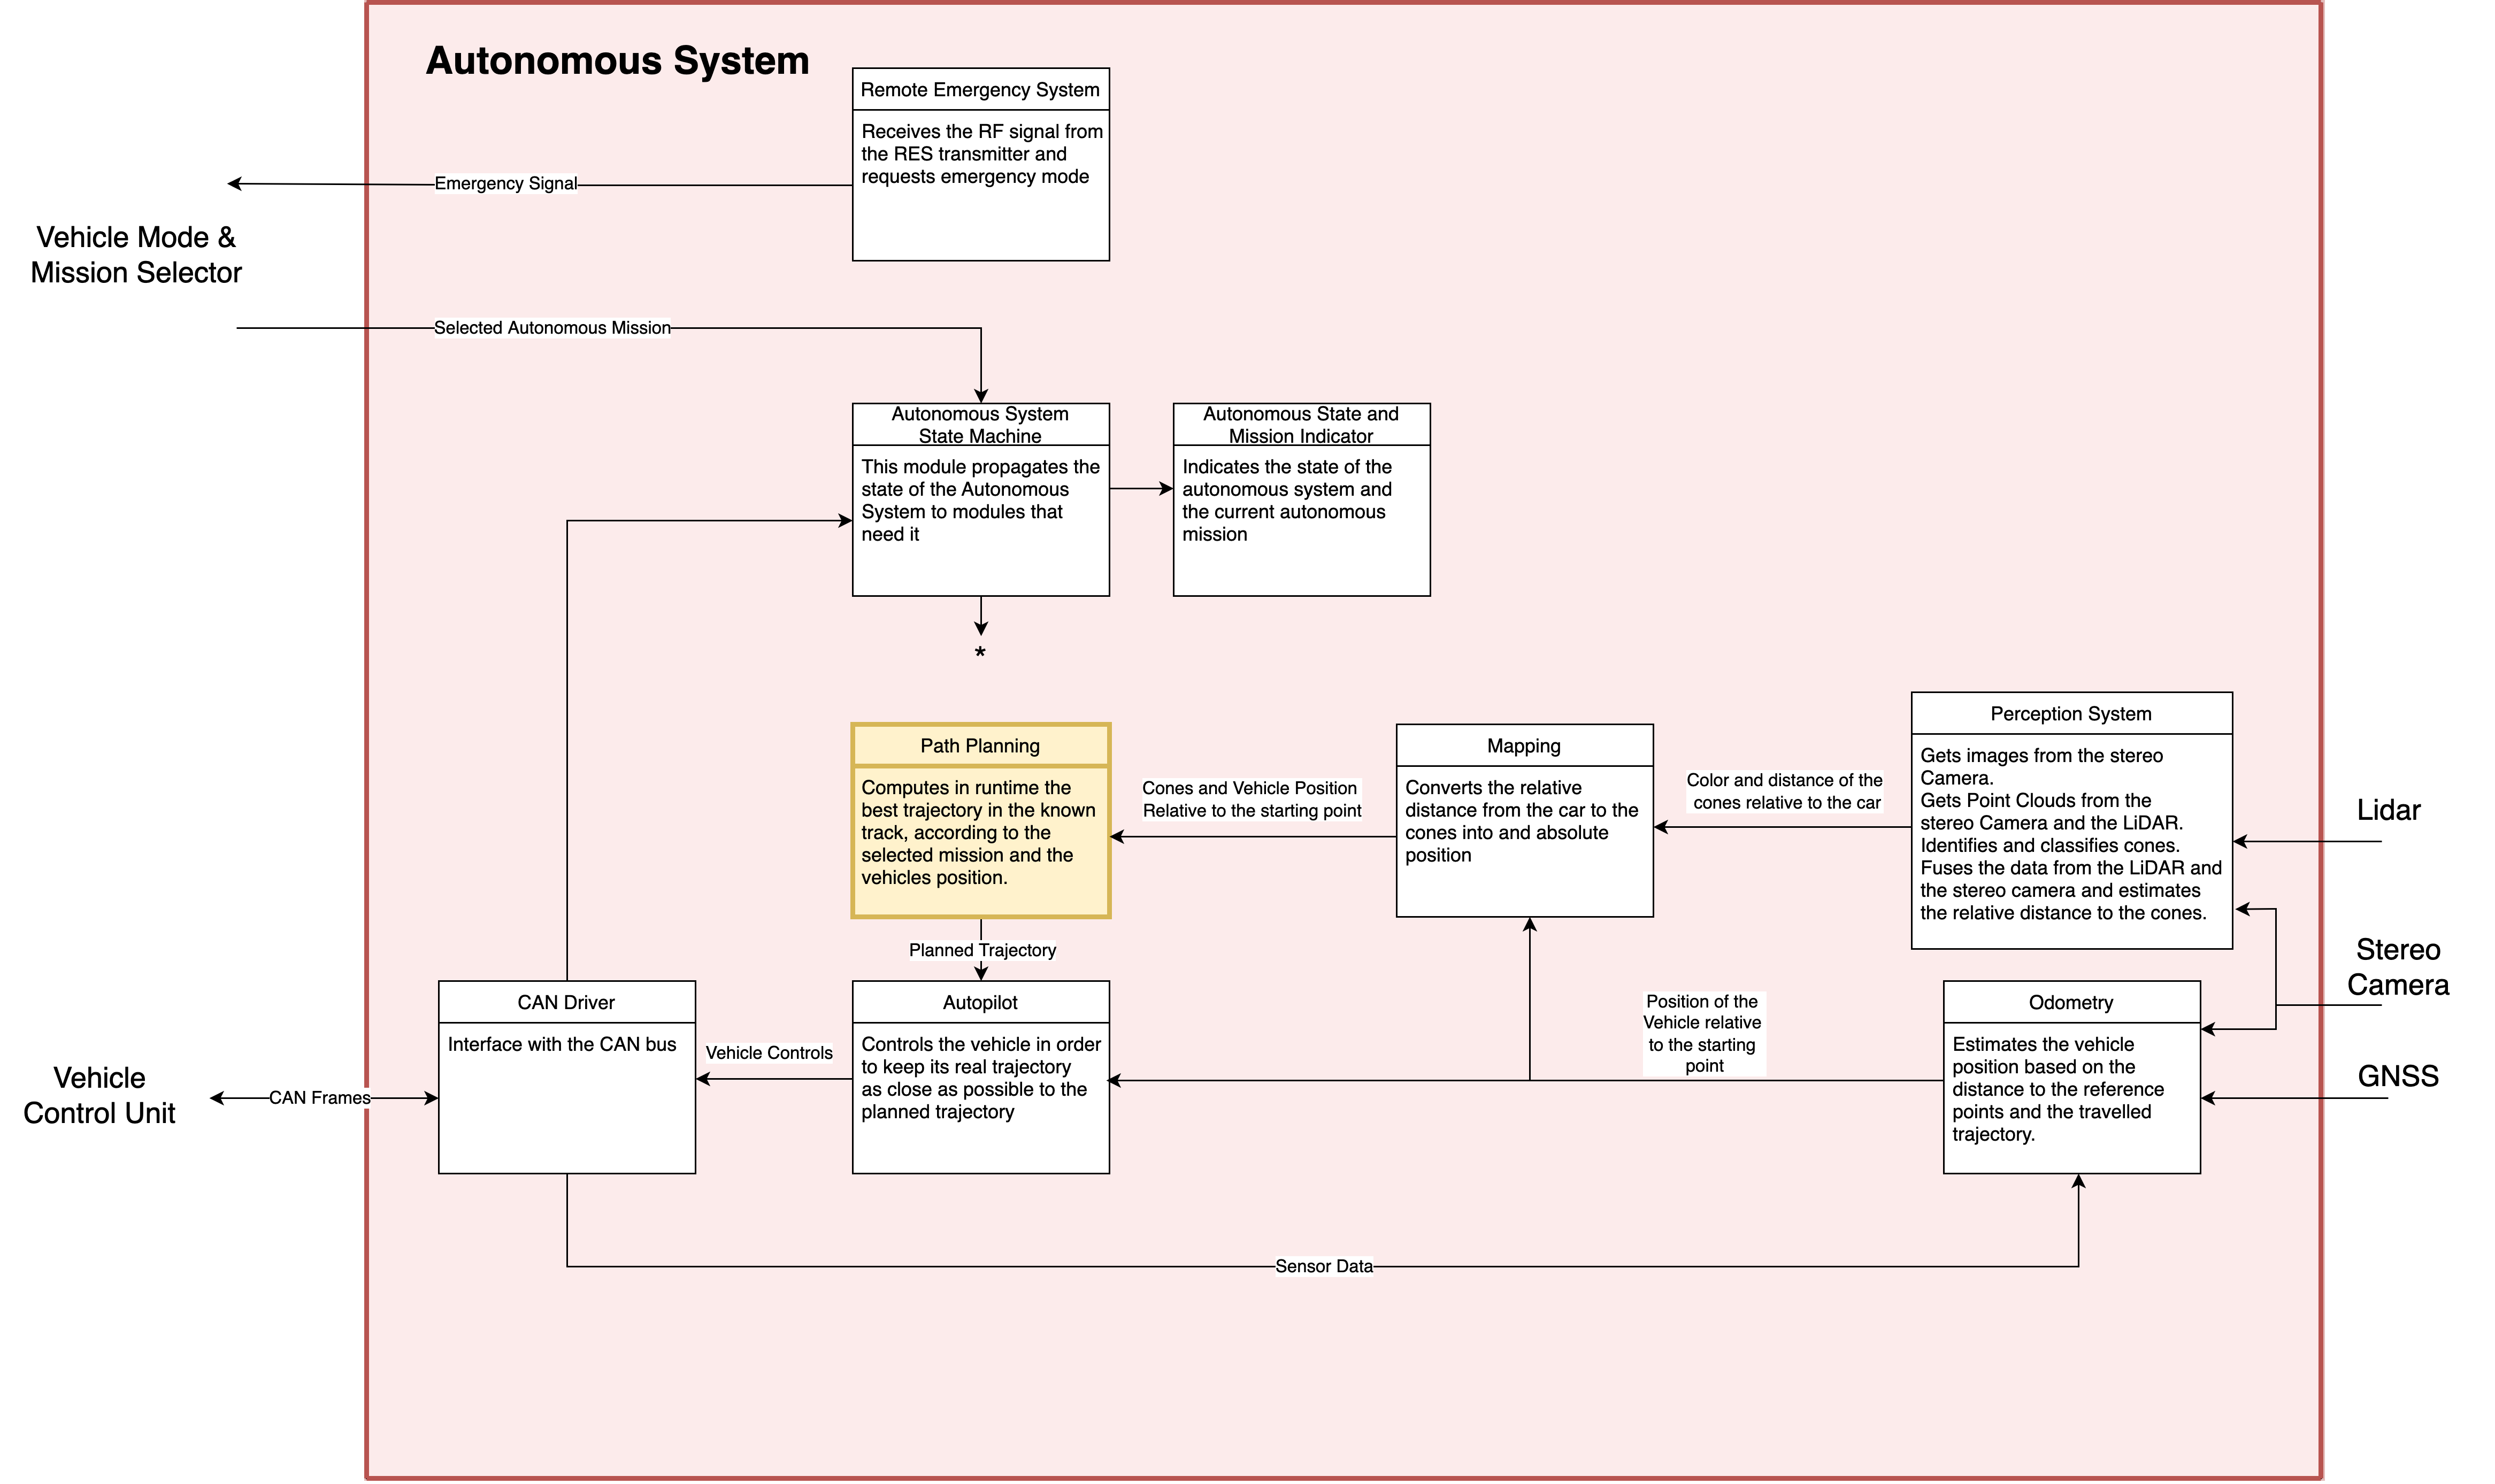
\includegraphics[width=\columnwidth]{AS_Component_Diagram.png}
    \caption{Autonomous System Component Diagram}
    \label{fig:AS Component Diagram}
\end{figure}
On a high-level view, the 'Autonomous System' is made up of five domains: 'Controls', which is responsible for the steering, breaking and acceleration of the car, 'Perception', which is responsible for the recognition of the track by perceiving the different types of cones the track is made up of, 'Localization and Mapping', which estimates the current position of the vehicle relative to the starting position and maps it into an absolute position on the track, 'Path Planning', which is responsible for the computation of the best possible path along the track, and 'Simulation', which is responsible for providing the rest of the domains an adequate tool to simulate and test on.
\begin{figure}[H]
    \centering
    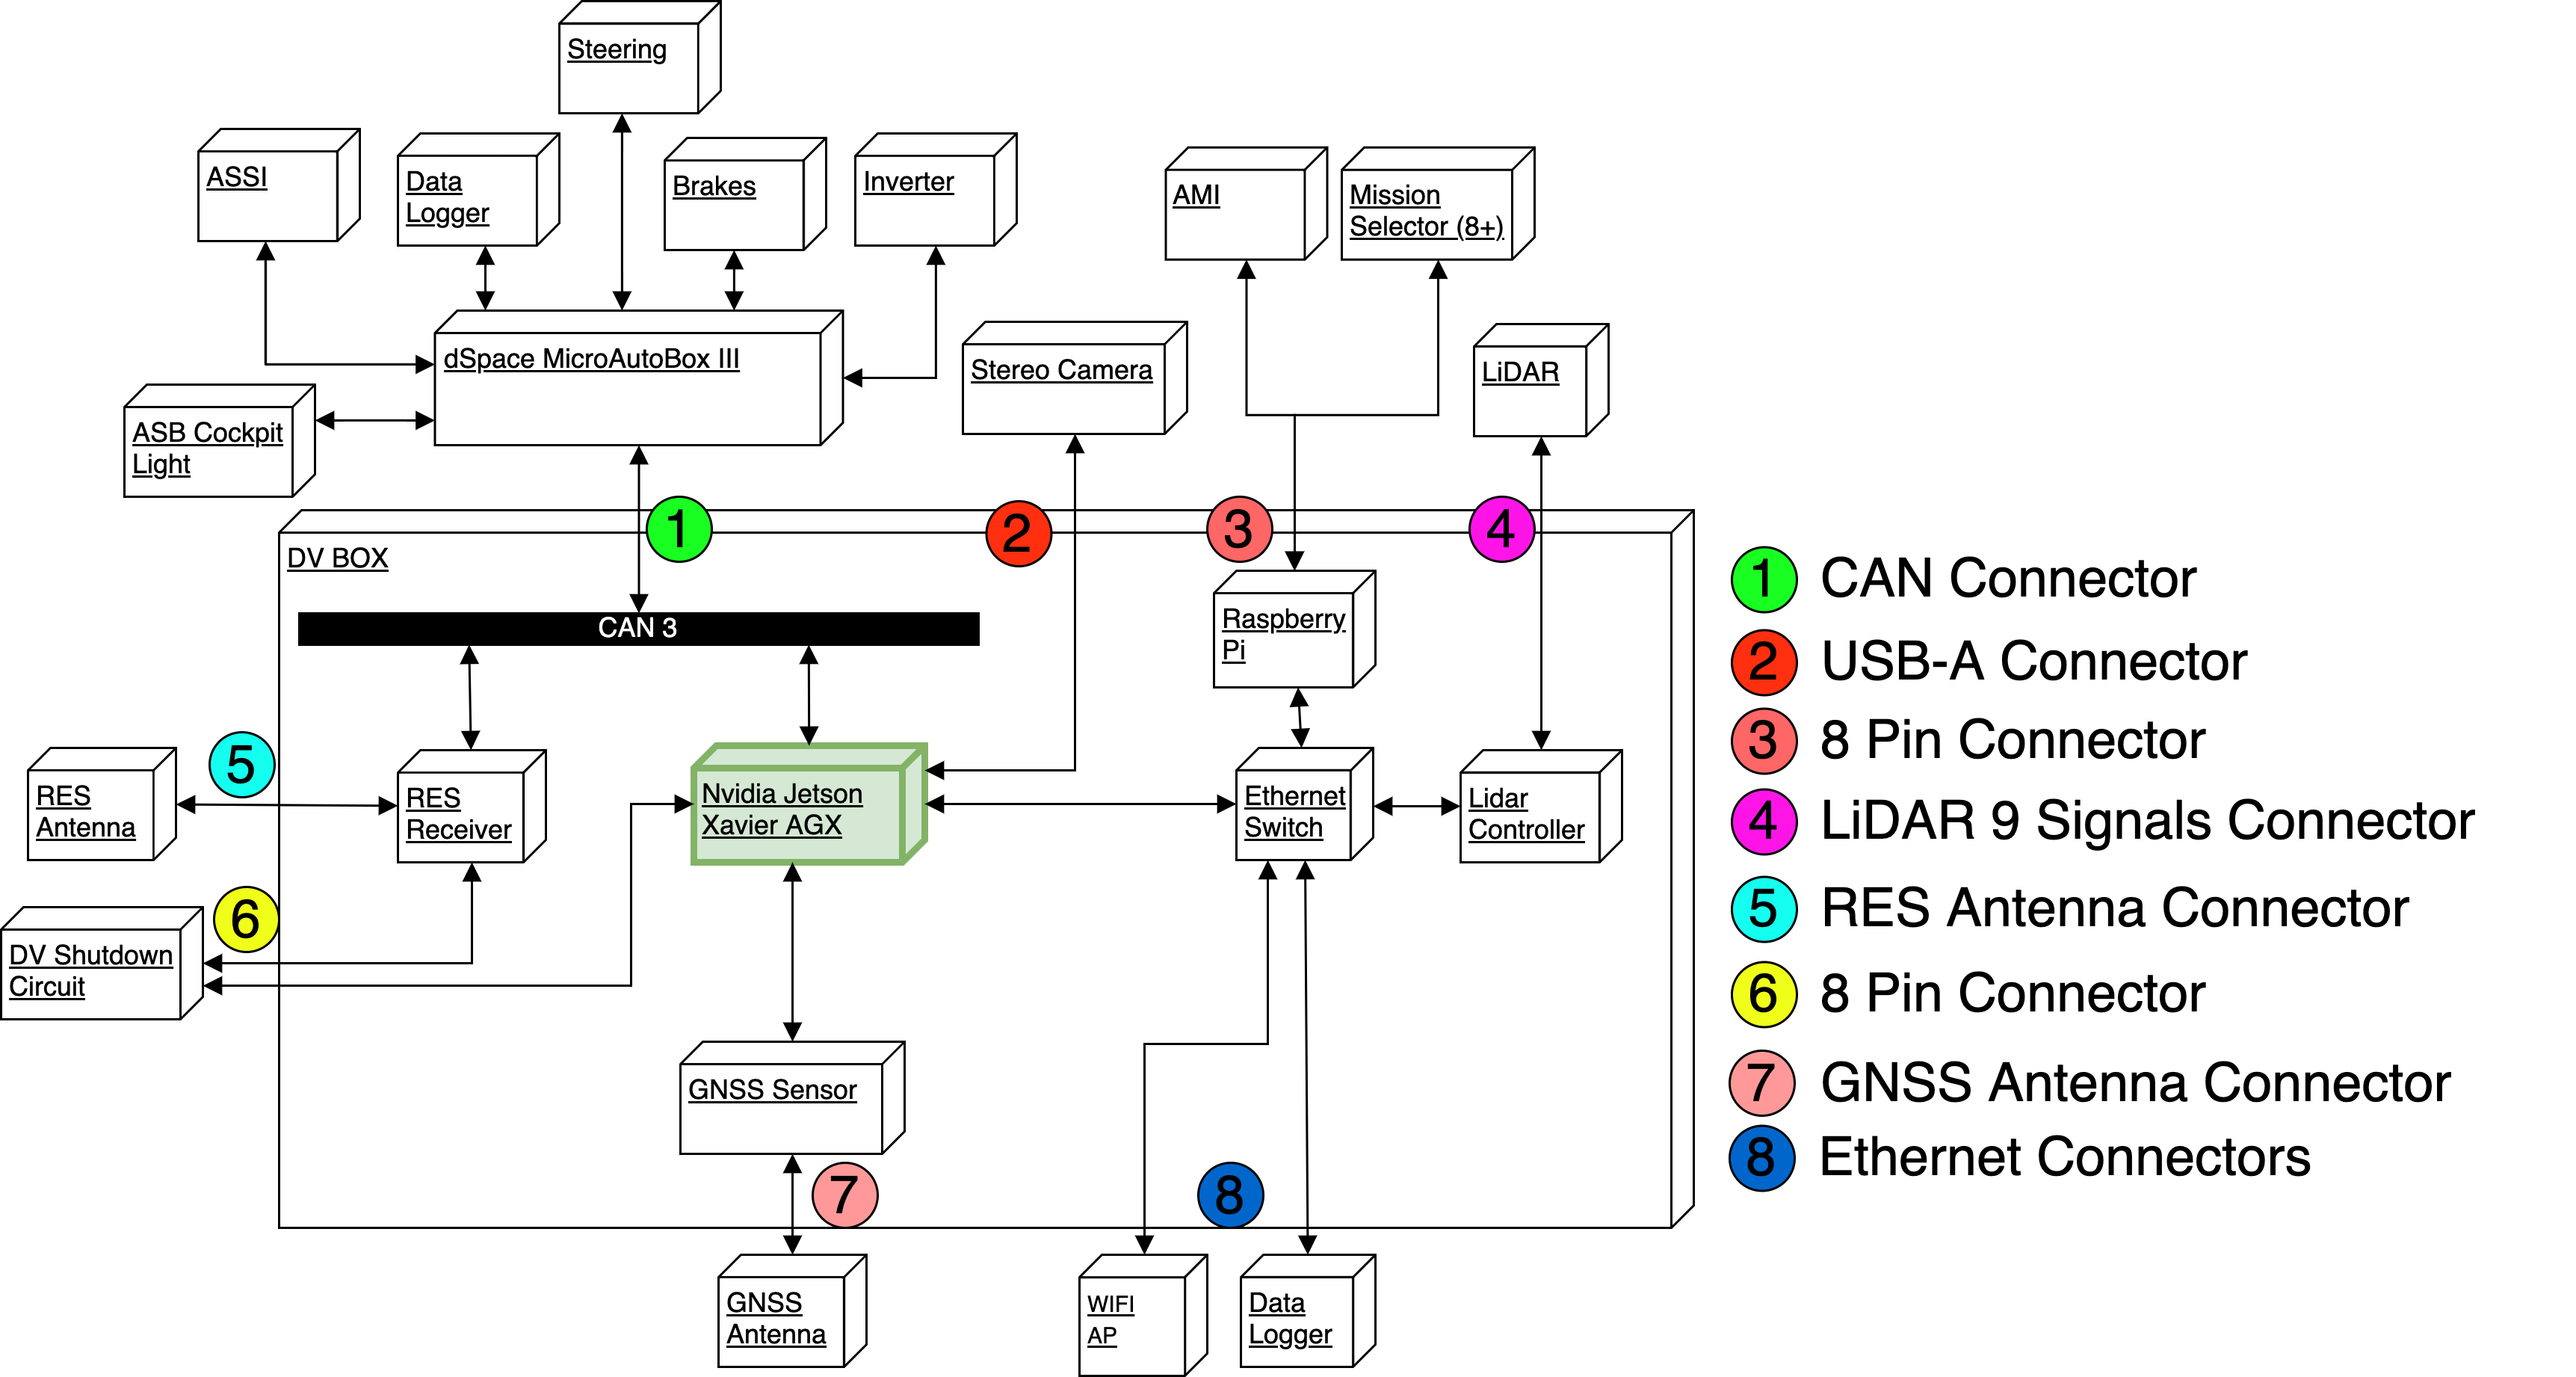
\includegraphics[width=\columnwidth]{AS_DV_Box.png}
    \caption{Autonomous System DV Box}
    \label{fig:AS DV Box}
\end{figure}

Essential hardware components of the autonomous system are stored inside a box, which will be mounted on the vehicle itself. The connections coming into the box from the various components outside can be seen in the reference diagram \ref{fig:AS DV Box}. Data needed for 'Localization' is received from the \acrshort{gnss} sensor and antenna (a MIKROE GNSS 7 Click and a u-blox ANN-MB), while the inputs for 'Perception' are received from the stereo camera (a Stereolabs ZED 2) and Lidar sensor (a Velodyne Lidar Puck Hi-Res), which both are also needed for the 'Path Planning' module. Information for the 'Control' unit are sent over to the engine control unit (ECU) (a dSPACE MicroAutoBox III). In the end, all critical data for the operation leads into the processing unit of the system, which is in this case a 'Jetson AGX Xavier' by NVIDIA. The Jetson is an AI computer which is made for autonomous machines in mind, delivering workstation performance in an embedded module under 30 Watts of power.
\begin{figure}[H]
    \centering
    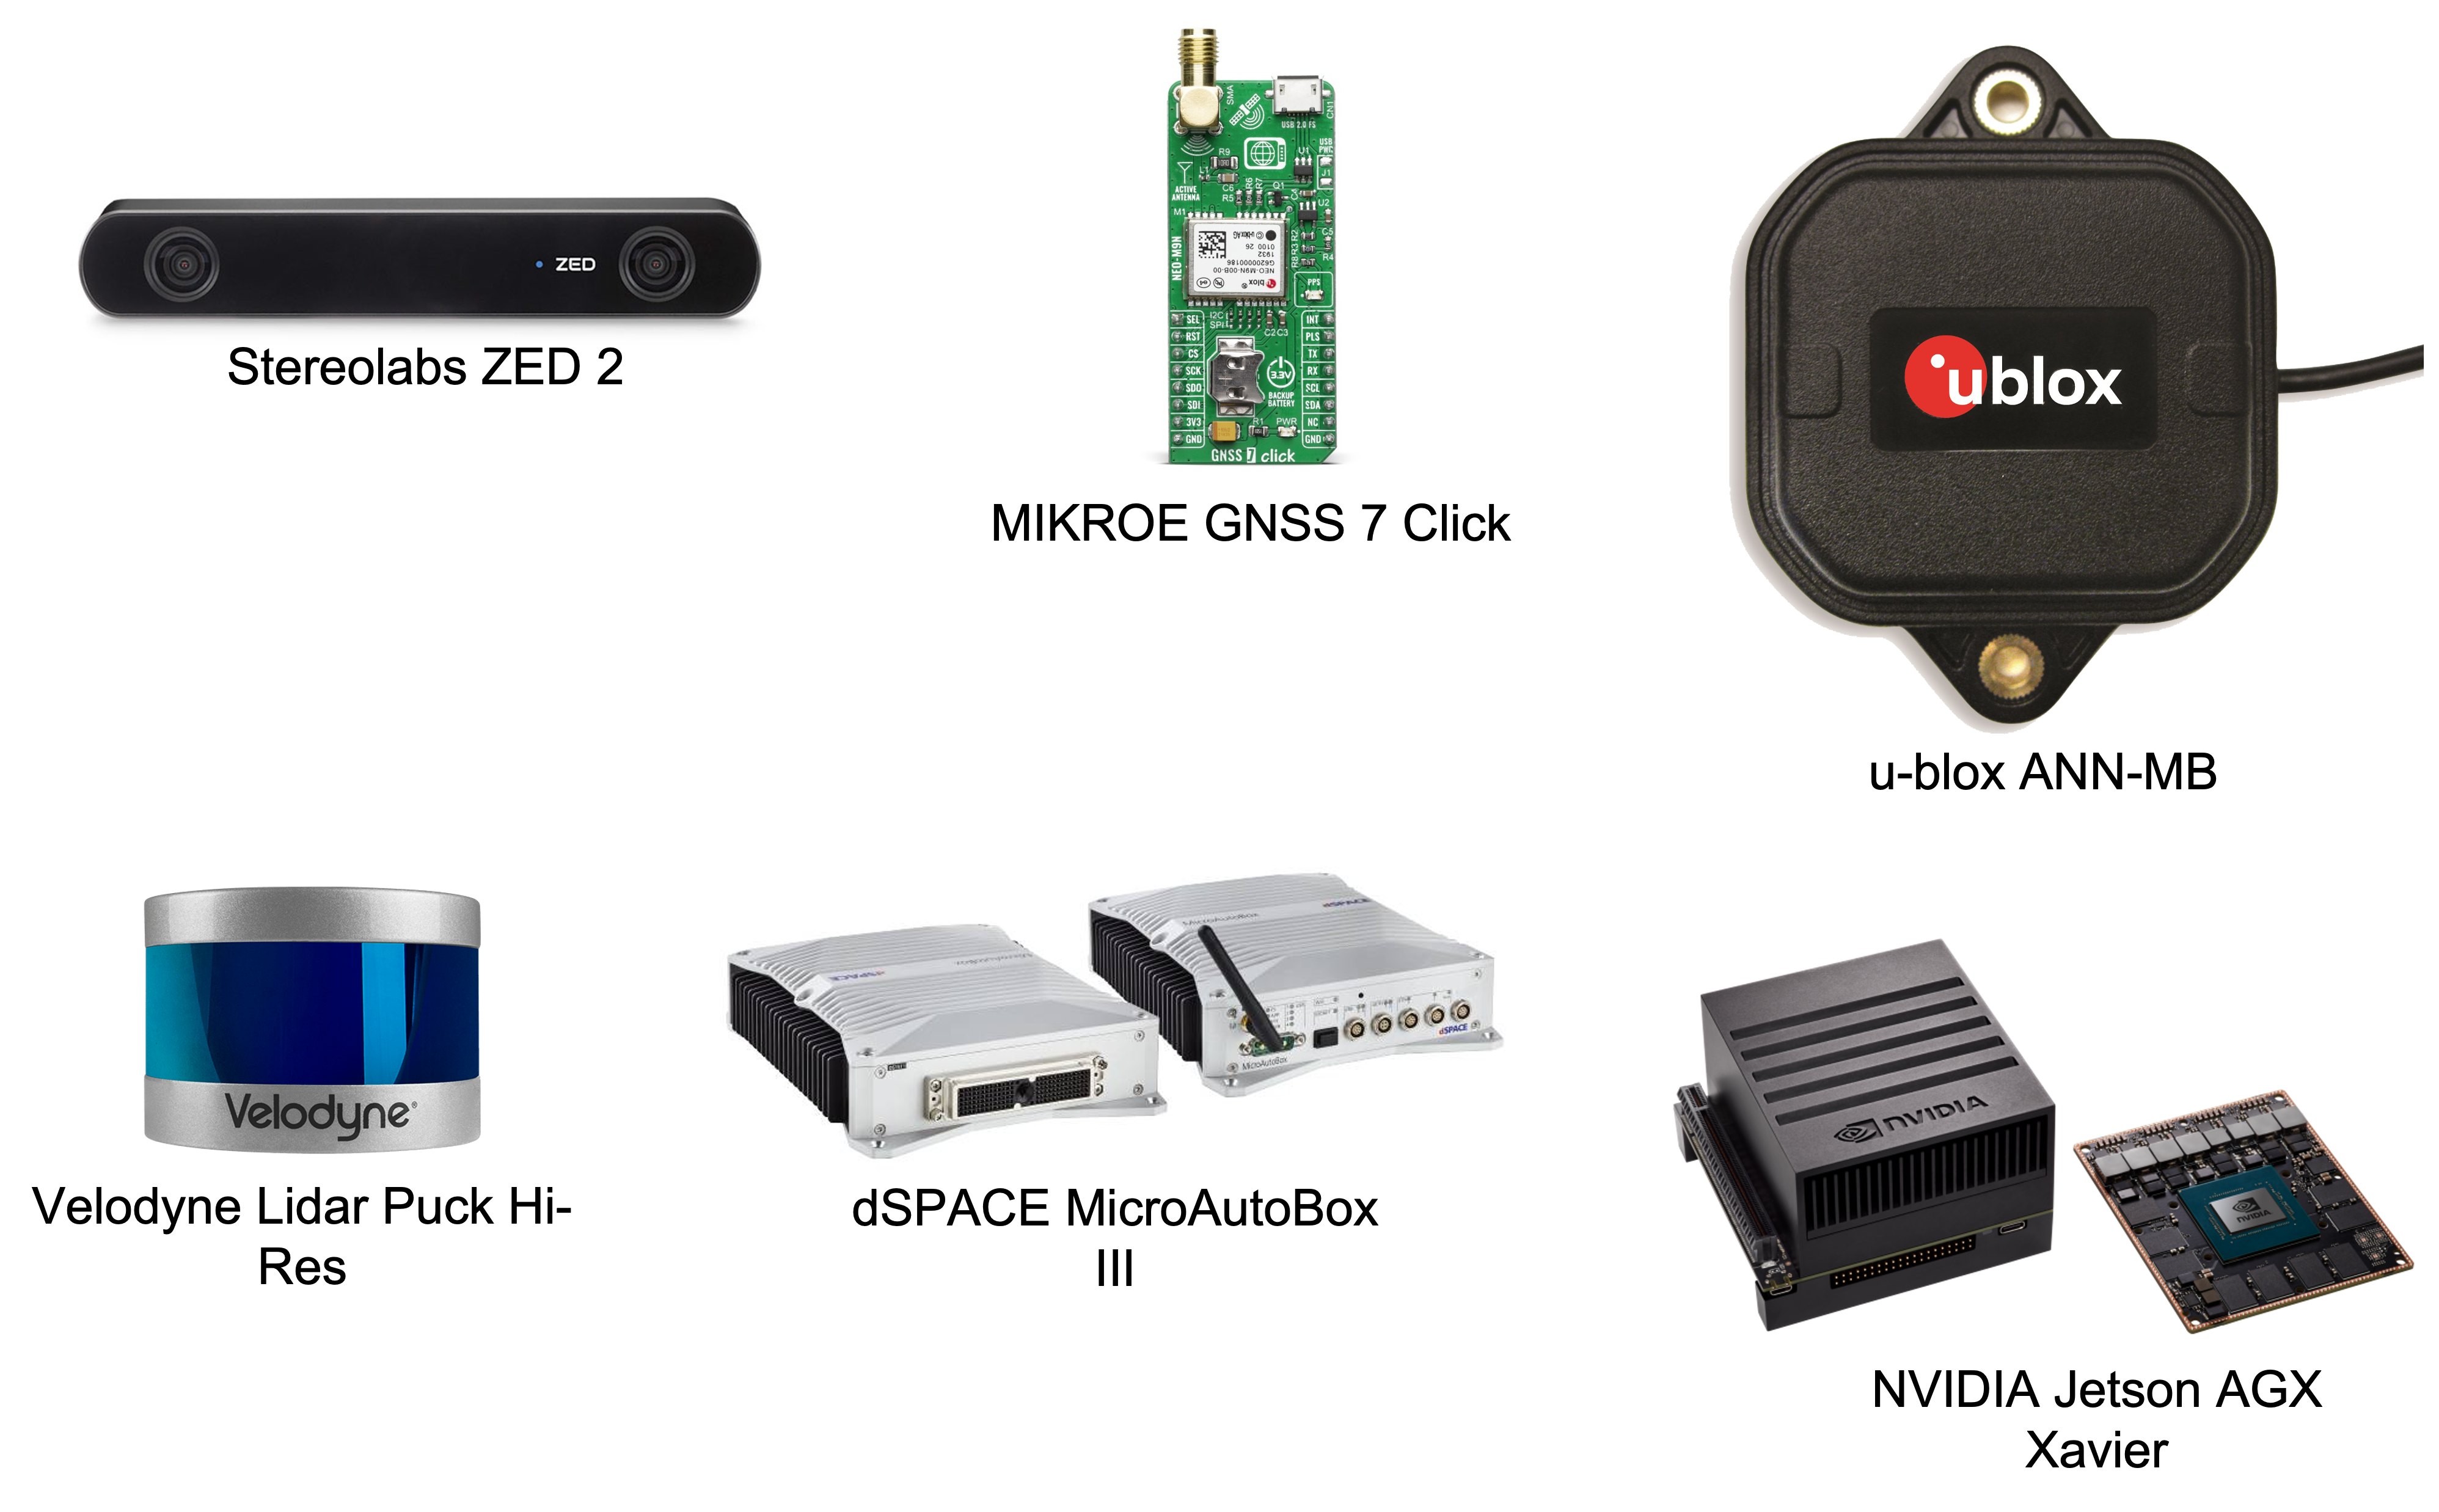
\includegraphics[width=\columnwidth]{AS_HW_Components.png}
    \caption{Autonomous System Hardware Components}
    \label{fig:AS HW Components}
\end{figure}

The processing unit is set up with an installation of Linux, which will run the software of the autonomous system on top of \acrshort{ros}.
\begin{figure}[H]
    \centering
    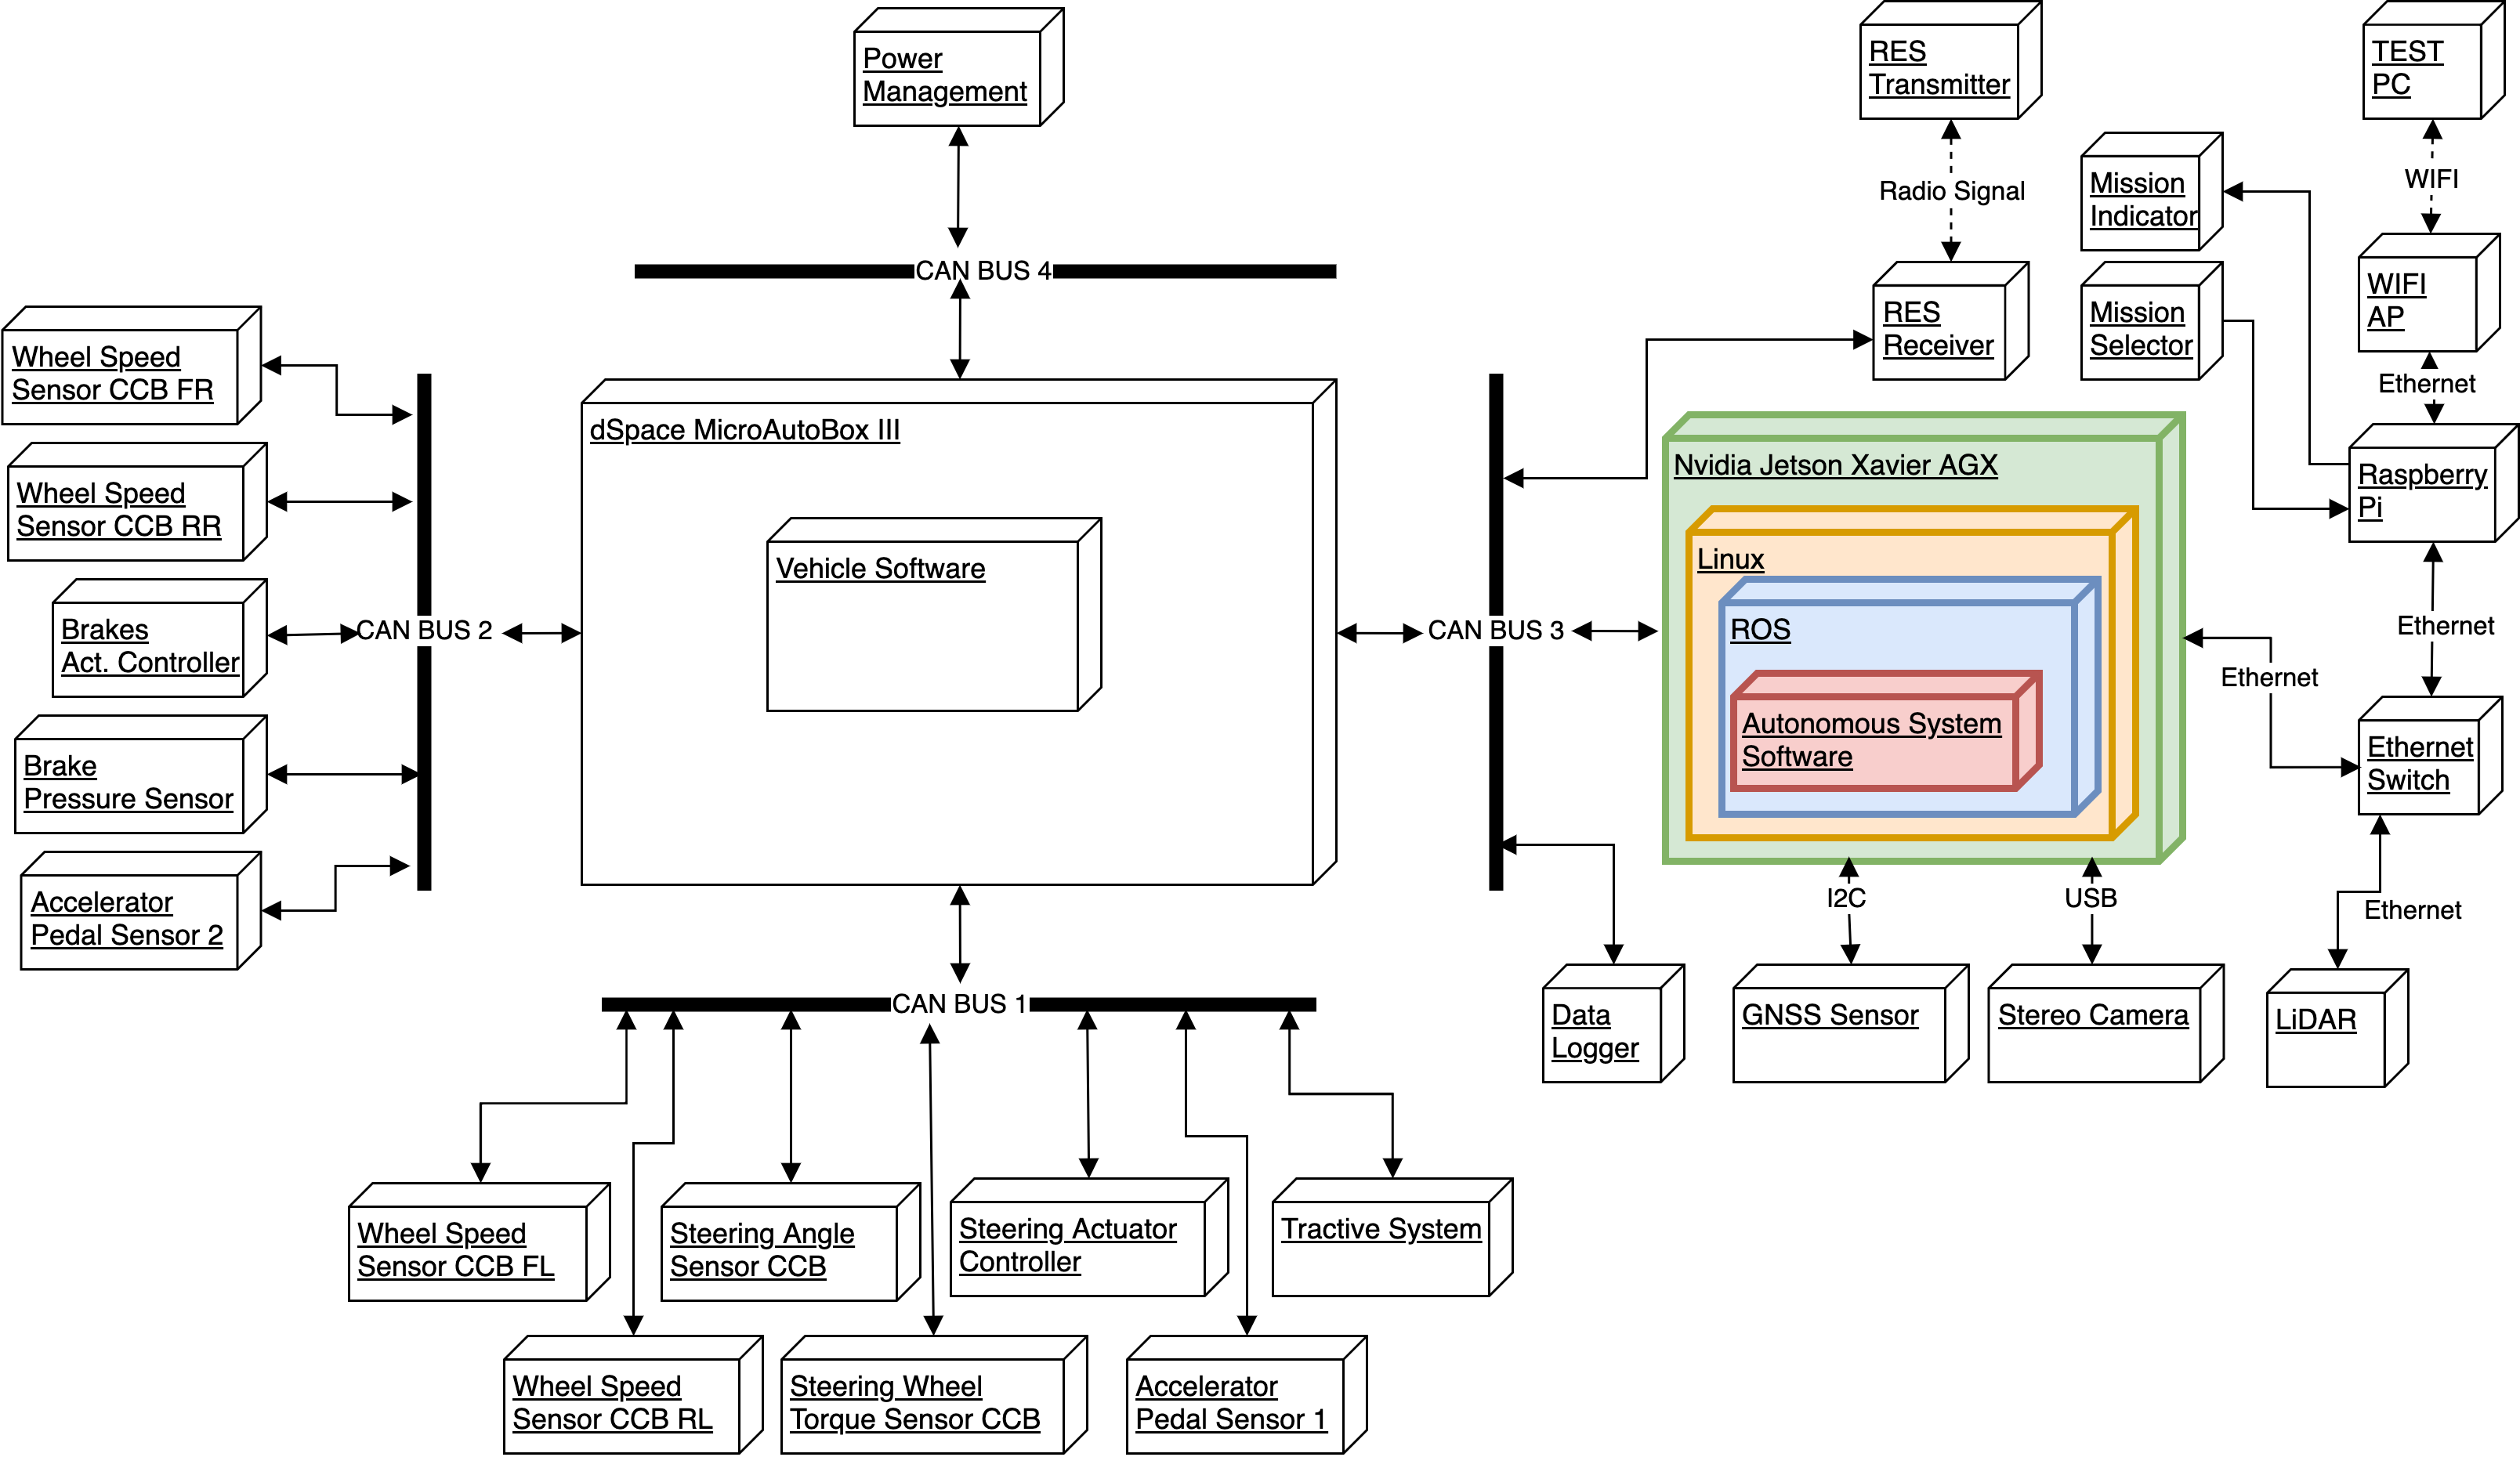
\includegraphics[width=\columnwidth]{AS_Deployment_Diagram.png}
    \caption{Autonomous System Deployment Diagram}
    \label{fig:AS Deployment Diagram}
\end{figure}

\section{Robot Operating System (ROS)}
The \acrlong{ros} (\acrshort{ros}) is not, like the name may suggest, a full-fledged operating system, but a set of software libraries and tools for the development of robot applications. The open-source robotics middleware comes shipped with capable developer tools, drivers and advanced algorithms. \cite{ros2_documentation}

There are currently two major versions of \acrshort{ros} which are seeing releases, ROS 1 and ROS 2. \cite{ros2_distributions} Beginning with releases after 'Foxy Fitzroy', releases in odd years will be non-LTS (Long Term Support) and will only be supported for 1.5 years, while new releases in even years are going to be long-term supported and will be supported for 5 years. \cite{ros2_releases_and_target_platforms}

The work done in this thesis have been done using the ROS 2 release 'Foxy Fitzroy', released on June 5th, 2020. This release will be supported till the end of May 2023. \cite{ros2_distributions}

\subsection{ROS Graph}
There are 5 main concepts of ROS 2 that make up the ROS (2) graph:
\begin{enumerate}
    \item Nodes
    \item Topics
    \item Services
    \item Parameters
    \item Actions
\end{enumerate}

The ROS graph is a network of ROS 2 elements which processes data simultaneously. The graph encompasses all executables and the connections between them.

\begin{figure}[H]
    \centering
    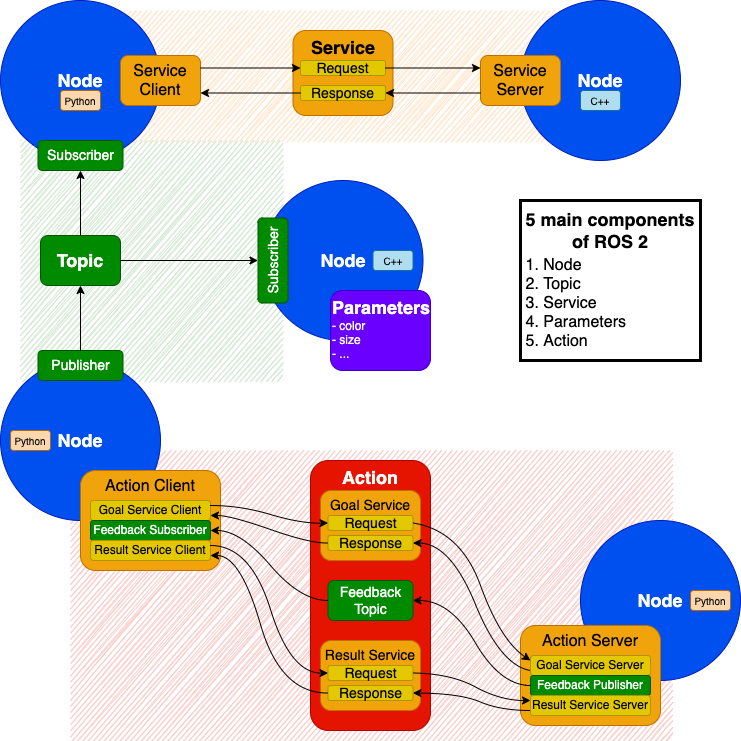
\includegraphics[width=\columnwidth]{ROS2_Main_Concepts.png}
    \caption{The five main concepts of ROS 2 pictured as a network of nodes.}
    \label{fig:ROS 2 main concepts}
\end{figure}

\subsubsection{Nodes}
A node is a fundamental ROS 2 element that serves a single, modular purpose in a robotics system. \cite{ros2_tutorials_nodes}

\subsubsection{Topics}
 Nodes publish information over topics, which allows any number of other nodes to subscribe to and access that information. \cite{ros2_tutorials_topics}

\subsubsection{Services}
Services are based on a call-and-response model, versus topics’ publisher-subscriber model. Services only provide data when they are specifically called by a client. \cite{ros2_tutorials_services}

\subsubsection{Parameters}
Nodes have parameters to define their default configuration values. \cite{ros2_tutorials_parameters}

\subsubsection{Actions}
Actions are built on topics and services and consist of a goal, feedback, and a result. Actions are like services that allow you to execute long-running tasks, provide regular feedback, and are cancellable. \cite{ros2_tutorials_actions}

\section{Driverless}
\lipsum[1]

\section{Path Planning Algorithms}
Path planning algorithms are used in many environments for example in assembling a car with a robot arm, parking a car autonomously or finding a landmine with a robot in a military operation. 

\subsection{Overview}
A path can be if a human goes from A to B and follows certain signs for example when hiking on a mountain. Otherwise, a human can follow a path that is generated on a GPS system in a car. The difference lies by a manual plan versus a generated plan by a machine. This section addresses only the generated one.

The planning consists of a state, time that is needed, actions, initial / goal state, criterion and a plan. The state is normally represented by a planning algorithm. Time is based on a sequence of decision that has to be made in a certain time. Actions manipulate the state and cover how the state should be changed. The initial and goal state defines where the planner should start and finish.
The criterion defines the outcome and the boundaries of the planner. The type of the criterion is either based on the feasibility or optimality. Feasibility covers the arrival of the goal state without the concern of efficiency. Optimality finds a plan with an optimized performance in mind. The plan in general covers the strategy or behaviour on a decision maker.
\cite{planning_algorithms_steven_m_lavalle_1_23}

\subsection{Algorithms, Planners and Plans}
An algorithm usually consists of a machine and environment where there are actuations from the machine to the environment and sensing from the environment to the machine.
\begin{figure}[H]
    \centering
    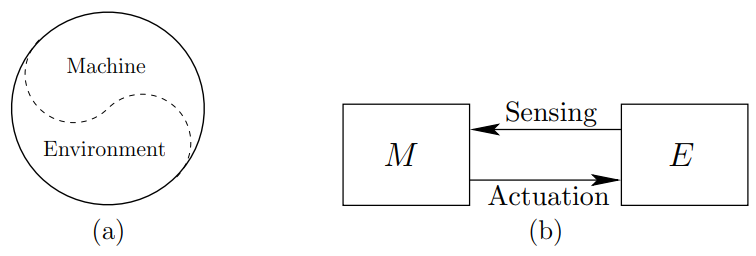
\includegraphics[width=\columnwidth]{Machine_Environment.png}
    \caption{Two different illustration to show what is the relationship between the machine and the environment. \cite{planning_algorithms_steven_m_lavalle_20}}
    %\label{fig:ROS 2 main concepts}
\end{figure}
The problem in planning is often that the machine interacts with the physical world which has uncountable different influences on the plan that has to be calculated. This is why the environment is often an approximation of the real world since not every sensing mechanism from the environment to the machine can be processed.

Planners are constructing plans. They are either a machine or a human. When the planner is a machine then it is usually a planning algorithm. If the planner is a human then the human itself is the algorithm which makes the decision.
\begin{figure}[H]
    \centering
    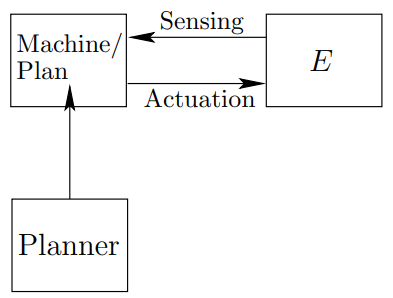
\includegraphics[width=\columnwidth]{Planner_Machine_Environment.png}
    \caption{A planner executes the plan on the machine that actuates on the environment. \cite{planning_algorithms_steven_m_lavalle_22}}
    %\label{fig:ROS 2 main concepts}
\end{figure}

The plans can be used in three different ways: Execution, refinement or hierarchical inclusion. Execution runs the plan on a simulation or a robot which is connected to the real world. Refinement tries to find a better plan. The hierarchical inclusion gives the plan to a higher level plan that is consisting of sub plans.

\cite{planning_algorithms_steven_m_lavalle_1_23}

\subsection{Path Planning Algorithm Categories}
A path planning algorithm can be categorized in one of the following groups:
\begin{itemize}
    \item Motion Planning
    \item Decision-Theoretic Planning
    \item Planning under Differential Constraints
\end{itemize}

\cite{planning_algorithms_steven_m_lavalle}

\subsubsection{Motion Planning}

Motion planning is interested in planning in continuous state spaces. This means that the space is not static and changes in relation to time. IT is also called motion planning or planning in continuous state spaces.

\textbf{Implicit Representation} of a state space in motion planning must be dealt with in planning algorithms. Implicit representations become more important in motion planning as the state space is uncountably infinite. It also tries to define 2D and 3D geometric models and transforms them. State spaces arise from these problems.

\textbf{Continuous $\rightarrow$ discrete} is the central theme in motion planning to transform models. Motion planning also covers combinatorial motion planning, which means with the input model the algorithm builds a representation of the original problem. There is also the field of sampling-based motion planning.

\begin{itemize}
    \item \textbf{Geometric Representation and Transformation} to start defining a motion planning algorithm. It defines a body of a system in a space and how it transforms for example moves. Movements can be chained in a state.
    \item \textbf{The Configuration Space} is needed for the motion planning algorithm to define the space in which is a set of possible transformations that could be applied to a robot.
    \item \textbf{Sampling-Based Motion Planning} is a field in motion planning that covers sampling-based algorithms. Sampling-based planning algorithm are using a collision detection as a "black box" which is separated to geometric and kinematic models motion planning. There are two different types of algorithm models. First is the single-query algorithm which consists of a ($q_i,q_G$) pair as an input. $q_i$ defines the start and $q_G$ the end goal. In this strategy no precomputation is possible to make use of. 
    \begin{figure}[H]
        \centering
        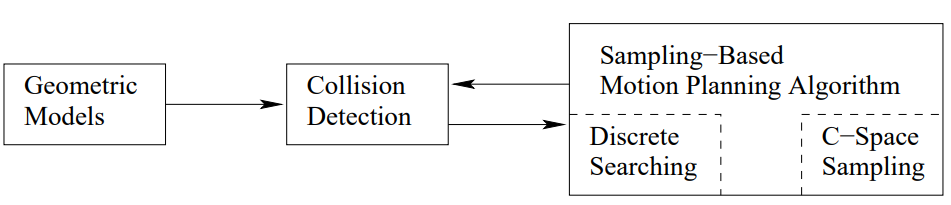
\includegraphics[width=\columnwidth]{Sampling-Based_Motion_Planning.png}
        \caption{The geometric models will generate the input for the collision detection, that influences the discrete searching in the sampling-based motion planning algorithm. The C-space is the configuration space of the algorithm. \cite{planning_algorithms_steven_m_lavalle_185}}
        %\label{fig:ROS 2 main concepts}
    \end{figure}
    A multi-query algorithm can have multiple initial goals, that is why it makes sense to precompute the models to run it more efficiently. An example of a single-query algorithm is the Rapidly Exploring Random Tree (RRT) which is a subset of the Rapidly Exploring Dense Tree (RDT) algorithm. It searches for the shortest path by creating random sequences that end up in a tree that holds multiple sequences which can be connected to each other. 
    \begin{lstlisting}[mathescape=true, caption={The simple RDT computes a random tree with the nearest function. \cite{planning_algorithms_steven_m_lavalle_229}}]
SIMPLE RDT($q_0$)
    1 G.init($q_0$);
    2 for i = 1 to k do
    3 G.add vertex($\alpha(i)$);
    4 $q_n \rightarrow$ nearest(S(G), $\alpha(i)$);
    5 G.add edge($q_n$, $\alpha(i)$);
    \end{lstlisting}
    The goal of the multi-query  method is to create a roadmap for each $q_i$ and $q_G$ that is why the family of algorithm is called sampling-based roadmap.
    \item \textbf{Combinatorial Motion Planning} covers finding a path in a continuous space without resorting to approximations. Cell decompositions and cylindrical algebraic decomposition are two different subcategories of combinatorial motion planning algorithms. Cell decompositions are based on a collection of cells that is called complex. The term cell decomposition describes a part of a complex which is a smaller number of cells in a space. In the 2D decomposition field there is the triangulation algorithm which is performed by vertical decomposition. The triangulation algorithm connects every build triangles with three nodes at a time. If you have 4 nodes then two triangles are made. 
    \begin{figure}[H]
        \centering
        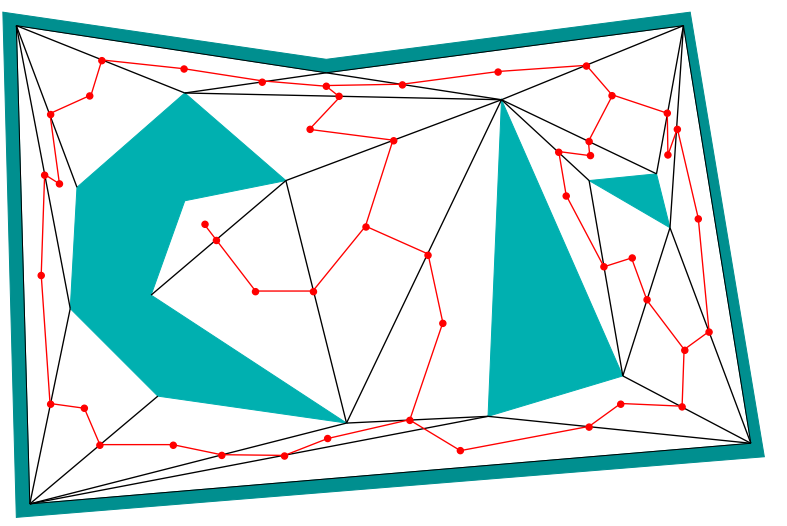
\includegraphics[width=\columnwidth]{Theorie_of_Triangulation.png}
        \caption{The black lines represent the triangles which are computed. The red dots on the other hand represent the middle point of the edges and the triangle itself. The red lines have the red dots as a reference point and can build a path. \cite{planning_algorithms_steven_m_lavalle_268}}
        %\label{fig:ROS 2 main concepts}
    \end{figure}
    In computational algebraic geometry the definition is very general that is why it can cover a lot of solution for problems but at the same time is challenging to implement. The definitions are described in tarski sentences. There are problems that can exist with this method the decision problem and the quantifier-elimination problem. To explain each problem would be out of scope. The Canny's roadmap algorithm a subset of computational algebraic geometry algorithm covers the avoidance of doubly exponentially cells in cylindrical algebraic. The result is that the algorithm can be run in polynomial time. The complexity of motion planning describes if it makes sense for an algorithm to be programmed more complexed or leave it as it is because timewise or storage wise it is not a drawback. Optimal motion planning is different to feasibility as it covers to find an optimal solution of the problem. It deals with finding an approximation of a continuous problem as a discrete problem.
    \item \textbf{Extensions of Basic Motion Planning} defines flavours of motion planning algorithms. There are for example the time-varying problems which are defined in a planning formulation. Time-varying problems consider time in the planning formulation. For example obstacles can change during time and the space would not be considered as static. Solutions for that are either sampling-based, combinatorial methods or bounded speed. Further more there can be multiple robots in a space. With multiple robots it is possible to combine the information of each robot so that one can benefit from the other. Otherwise, there is also the problem that the robots do not collide with each other. Euclidean shortest path algorithm gives a solution for solving a motion plan.
    \item \textbf{Feedback Motion Planning} describes a class of motion planning algorithms that are taking feedback for example from the real world into account. With the help of the Dijkstra algorithm an optimal navigation function can be programmed to work in a feedback motion planning environment with acceleration in consideration for example.
\end{itemize}

\cite{planning_algorithms_steven_m_lavalle_77_432}

\subsubsection{Decision-Theoretic Planning}

This chapter can also be called planning under uncertainty. Two aspects evolve under uncertainty: predictability and sensing. It could also mean that an algorithm has to interfere with another decision maker. Instead of making a plan in decision-making, the chapter covers strategies that for a decision maker. Nature can be a decision maker as well. While it is possible to predict certain things about nature the factors of the interference of nature is still too big. That is why while programming an algorithm the programmer has to concentrate on the earthly influence which has the biggest impact of the robot or so-called primary decision-maker.

\begin{itemize}
    \item \textbf{Sequential Decision Theory} deals with forward and backward projections. A forward projection predicts how the future route will look like and the backward projection. Forward projection is a method where several possible stages are computed before it decides which path to go. Back projection is the other way around. With the help of graph search it is possible to have a more stable solution for calculating a path then with other methods like value iteration or policy iteration. With the help of the Dijkstra algorithm it is improved with less cost to calculate. Infinite-horizon problems can occur when dealing with algorithm under the sequential decision theory. Reinforcement Learning helps to solve the inifinite-horizon problem in combination with the optimal path in one algorithm.
    \item \textbf{Sensors and Information Spaces} describes how the sensors act and the planning problem witch is described as an information space. There are discrete state spaces and derived information spaces. Sensors have two components, the observation space that defines possible states and a sensor mapping which is what the sensor reads.
    \item \textbf{Planning Under Sensing Uncertainty} covers algorithms which can be used to plan under sensing uncertainty. Localization as a problem in robotics can be hard to accomplish. There is the passive localization and the active localization. In passive localization a robot acts upon different circumstances and derives its position from probabilistic approaches whereas active localization the focus is more on how the robot should move to be in that exact position. 
    \begin{figure}[H]
        \centering
        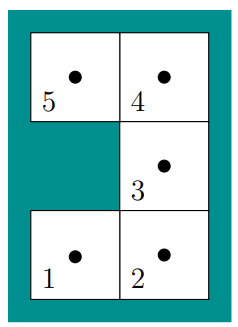
\includegraphics[width=\columnwidth]{Localization_Example.png}
        \caption{This example shows possible moves of a robot to which grids he could move to. \cite{planning_algorithms_steven_m_lavalle_641}}
        %\label{fig:ROS 2 main concepts}
    \end{figure}
    
    With combination of different sensors like compass and a camera it is possible to define a position. Further information on localization can be read in the mentioned book. The environment uncertainty and mapping topic focuses on how to define an environment when there is no map given. This means that the robot has to act upon sensors only.
\end{itemize}

\cite{planning_algorithms_steven_m_lavalle_433_710}

\subsubsection{Planning under Differential Constraints}
This chapter covers differential constraints. These for example local limitation like allowable velocities at each point. A weak differential constraint is for example smoothness. Global constraints are for example obstacles. Mostly differential constraints are from kinematics and dynamics.

\begin{itemize}
    \item \textbf{Differential Models} covers example of velocity constraints in a state space. There are two ways to of differential constraints the parametric and implicit. Implicit expresses prohibited velocities and are more general whereas parametric representation expresses allowed velocities. A simple car has three degrees of freedom:
    \begin{figure}[H]
        \centering
        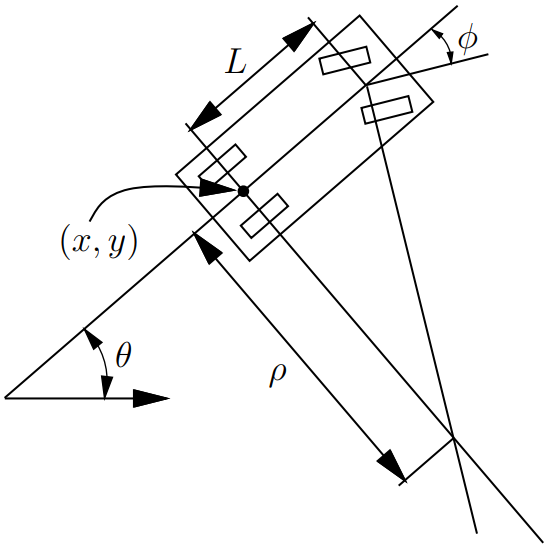
\includegraphics[width=\columnwidth]{Simple_Car_Velocity_Space.png}
        \caption{This example shows possible moves of a robot to which grids he could move to. \cite{planning_algorithms_steven_m_lavalle_723}}
        %\label{fig:ROS 2 main concepts}
    \end{figure}
    The velocity is two-dimensional on the other hand. This means that it has to be shrunken down from three dimensions to two. There are also concepts of multiple decision makers, which are not covered in this thesis.
    \item \textbf{Sampling-Based Planning Under Differential Constraints} covers the satisfaction of differential constraints with an initial and goal state. Constraints like continuity or smoothness can be applied as well. Kinodynamic planning is a motion planning problem with velocity and accelerations bounds. Trajectory planning on the other hand deals with a velocity and path function. There can also be collision constraints with obstacles for example.
    Reachable sets describe what has to be visited, there could also be time-limited reachable sets. A reachability graph can help to visualize which sets are already visited:
    \begin{figure}[H]
        \centering
        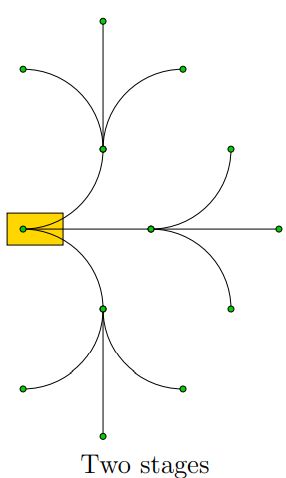
\includegraphics[width=\columnwidth]{Reachability_Graph.png}
        \caption{This figure shows how a reachability graph can be visualized. \cite{planning_algorithms_steven_m_lavalle_803}}
        %\label{fig:ROS 2 main concepts}
    \end{figure}
    Local planning by the having smaller problems which can be solved locally to solve the bigger problem. The following pseudo-code snipped shows how the rapidly exploring dense tree (RRT) can be used for calculating a path under differential constraints:
    \begin{lstlisting}[mathescape=true, caption={The local planning method computes $x_r$. A new vertex will be available: $x_r$.\cite{planning_algorithms_steven_m_lavalle_833}}]
SIMPLE RDT WITH DIFFERENTIAL CONSTRAINTS($x_0$)
    1 G.init($x_0$);
    2 for i = 1 to k do
    3 $x_n$ $\leftarrow$ nearest(S(G), \alpha(i));
    4 ($\widetilde{u}^p$, $x_r$) $\leftarrow$ local planner($x_n$, $\alpha(i)$);
    5 G.add vertex($x_r$);
    6 G.add edge($\widetilde{u}^p$);
    \end{lstlisting}
    Randomized potential fields can also be a method for sampling-based planning under differential constraints, which is not covered in this thesis. Path constraints can narrow down the trajectory as well, like the turning angle.
    \item \textbf{System Theory and Analytical Techniques} takes the physics of the robot into account. Since this thesis covers trajectory planning or path planning this section would be out of scope.
\end{itemize}

\cite{planning_algorithms_steven_m_lavalle_711_923}

\section{Languages and Tools}

\begin{itemize}
    \item ROS 2
    \item Python
    \item LaTeX
    \item Git
    \item VS Code
    \item Azure DevOps
    \item GitHub
    \item Simulation tools
    \item other tools
\end{itemize}

\lipsum[1]